\subsection{Compuertas LSTM y GRU}

Hasta el momento, se ha hecho mención de las salidas $o^{(t)}$ y estados ocultos $h^{(t)}$ solo como
el resultado de operaciones aplicadas por dos funciones; $g$ y $f$ respectivamente. Existen varias
alternativas de construir una \textit{RNN}, una de las maneras más comunes es usando
\ref{eq:rnn_Ht} y \ref{eq:rnn_Ot}:

\begin{equation}
    h^{(t)} = \phi(x^{(t)} W_{x} + h^{(t-1)} W_h + b)
    \label{eq:rnn_Ht}
\end{equation}

\begin{equation}
    o^{(t)} = x^{(t)} W_{out} + b
    \label{eq:rnn_Ot}
\end{equation}

Donde los parámetros compartidos de la red ahora son descritos por las matrices
$W_x \in \mathbb{R}^{d \times k}$, $W_h \in \mathbb{R}^{k \times k}$ y $
W_{out} \in \mathbb{R}^{k \times q}$ con $k$ como la dimensión del estado oculto, $q$ la dimensión
de las salidas $o^{(t)}$, $b \in \mathbb{R} ^ {1 \times q}$ el parámetro de sesgo y $\phi$ es la
función de activación. De esta manera, los pesos de los parámetros aprendidos en la matriz $W_h$
determinan cómo será usada la información del pasado, codificada en $h^{(t-1)}$. Posteriormente
es incluida a la codificación de la información del tiempo actual $t$ calculada por $W_x$. La figura
\ref{fig:rnn_cell} representa gráficamente la lógica usada para calcular los estados ocultos y las
salidas de la red.


\begin{figure}
\centering
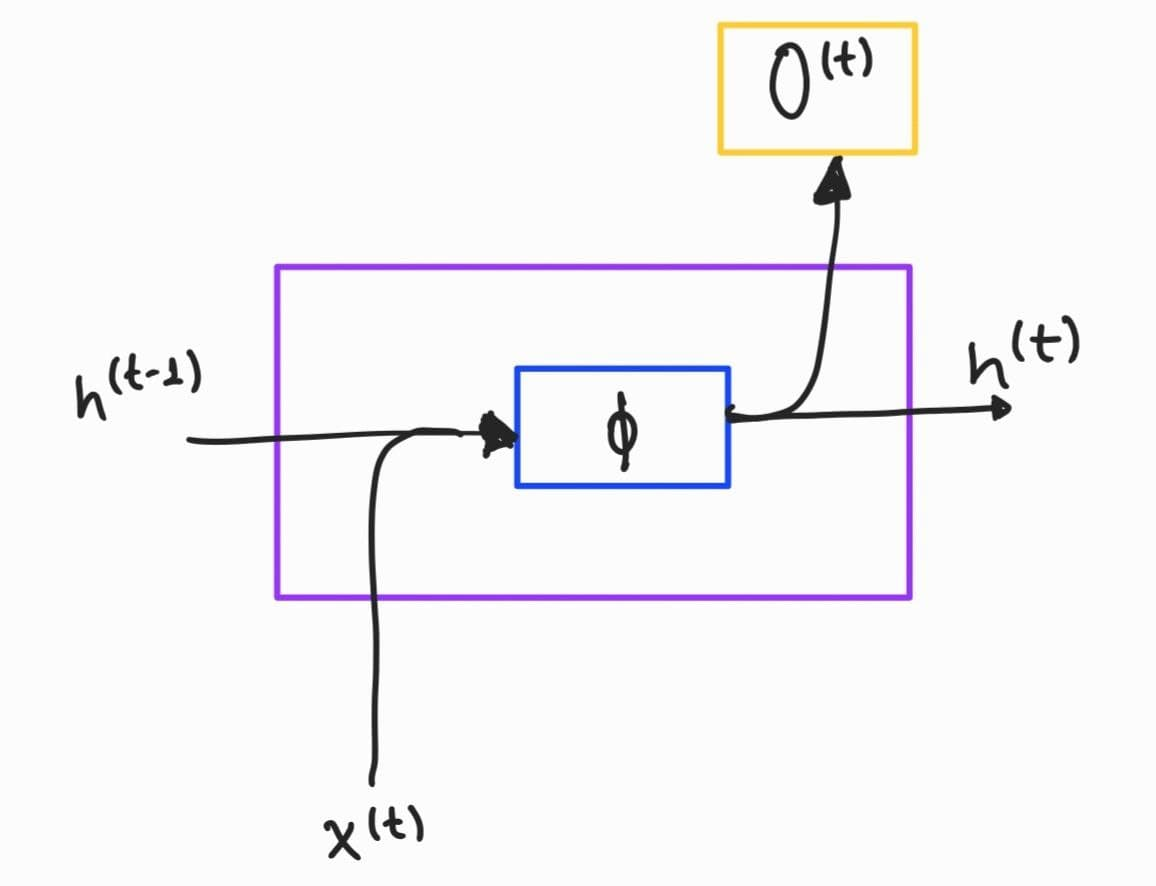
\includegraphics[width=0.4 \textwidth]{Chapters/1. Transformer/Figures/rnn/rnn_cell.jpg}
\caption{Computo del estado oculto y salida de una Red Neuronal Recurrente.}
\label{fig:rnn_cell}
\end{figure}

Sin embargo el cálculo de los estados ocultos mediante \ref{eq:rnn_Ht} presenta algunos problemas.
La interacción entre la información del pasado y la actual siempre es "plana", es decir, la información
fluye a través del tiempo de la misma manera sin forma de dar prioridad o ignorar parte de
esta. Por lo que resulta una tarea un poco más complicada preservar información relevante a en cada paso
o desechar información que ya no es util para la red. También, causado por este mismo flujo de los
datos, la información del pasado poco a poco es opacada por nueva información, impidiendo que se
puedan encontrar dependencias de información en secuencias largas en tiempos distantes;
comúnmente se hace referencia a este problema como \textit{The Short-term Memory Problem} en inglés
\cite{VanishinGradient2}.
Aunado a problemas como el
\textit{Desvanecimiento o Explosión del Gradiente} \cite{VanishinGradient} \cite{pmlr-v28-pascanu13},
acentuándose aun más
debido a las matrices de pesos compartidos en la recurrencia. Por ejemplo, podemos imaginar las
multiplicaciones en la recurrencia como un problema simplificado en donde dicha matriz es
multiplicada por si misma muchas veces (una similitud al método de potencia donde cualquier
componente en la matriz inicial que no esté alineada con el vector propio asociado al mayor valor
propio son eventualmente descartados \cite[pp.~390-392]{GoodBengCour16}), así los resultados de este producto
tendrán a ser cercanos a cero (desvanecerse) o explotar dependiendo de la magnitud de la matriz de pesos.

Una manera de solventar los problemas anteriores son las \textbf{Redes Neuronales con Compuertas},
creadas con la idea de crear conexiones a través del tiempo de tal manera de tener gradientes que no
se desvanezcan o exploten, convirtiéndose además en un mecanismo para olvidar información pasada y
decidiendo automáticamente cuándo y cuánto de la información debe prevalecer.

\subsubsection{LSTM}

\textbf{Long Short-Term Memory}, \textbf{LSTM} por sus siglas en inglés, fue propuesta en 1997 por
\textit{Hochreiter y Schmidhuber} \cite{LSTM}, como un método de preservar dependencias de información relevante
distantes a corto plazo. Las \textit{LSTM} introducen un nuevo componente la
\textit{Celda de Memoria} cuya función es guardar información a través del tiempo y es
controlada por distintas compuertas, las cuales aprenden a distinguir que información es relevante y
cual no. Contiene tres compuertas, la \textit{Compuerta de Entrada}, la \textit{Compuerta de Olvido}
y la \textit{Compuerta de Salida}. La \textit{Compuerta de Entrada} $I^{(t)}$ (véase la figura
\ref{fig:rnn_lstm}) determina cuanta información actual debe ser contemplada a través de la
\textit{Memoria Candidata} $\tilde C^{(t)}$ para actualizar la \textit{Celda de Memoria} $C^{(t)}$.
La \textit{Compuerta de Olvido} indica qué información del pasado debe ser desechada de la
\textit{Celda de Memoria} $C^{(t-1)}$ y la \textit{Compuerta de Salida} ayuda a determinar el nuevo
estado $h^{(t)}$ via la \textit{Celda de Memoria} actual $C^{(t)}$.

\begin{figure}[ht!]
\centering
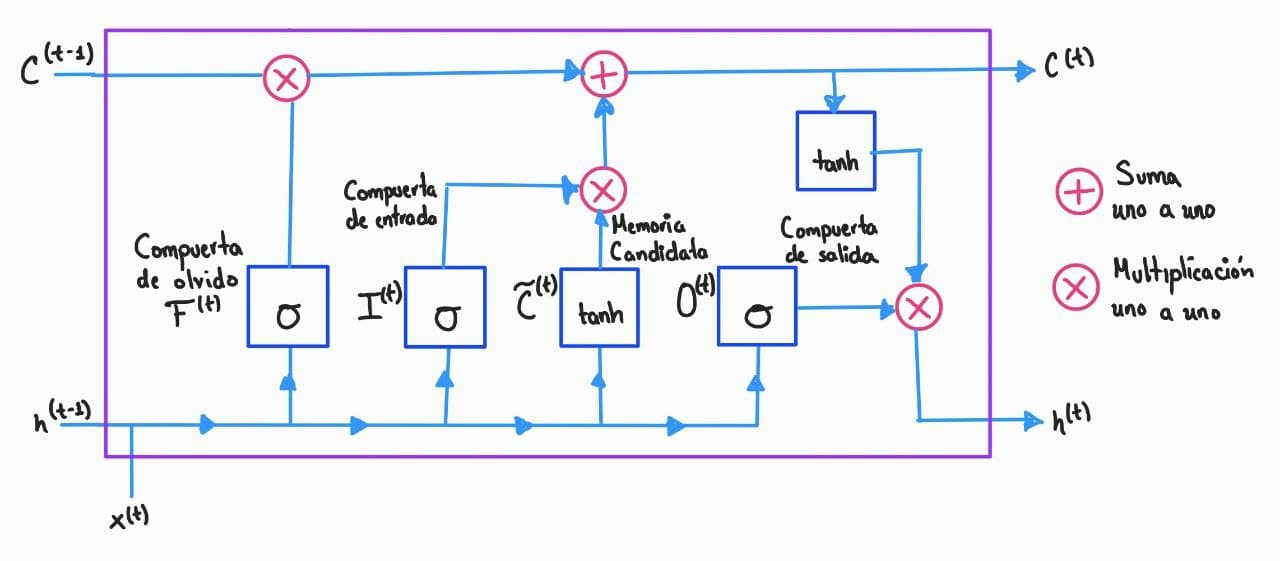
\includegraphics[width=1.0 \textwidth]{Chapters/1. Transformer/Figures/rnn/lstm.jpg}
\caption{Computo del estado oculto y salida de una Red Neuronal Recurrente.}
\label{fig:rnn_lstm}
\end{figure}

Las ecuaciones \ref{eq:comp} rigen el comportamiento de Compuertas de Entrada, Salida y Olvido.

\begin{equation}
    \begin{split}
        I^{(t)} =  \sigma(x^{(t)} W_{xi} + h^{(t-1)} W_{hi} + b_i)\\
        F^{(t)} =  \sigma(x^{(t)} W_{xf} + h^{(t-1)} W_{hf} + b_f)\\
        O^{(t)} =  \sigma(x^{(t)} W_{xo} + h^{(t-1)} W_{ho} + b_o)\\
    \end{split}
    \label{eq:comp}
\end{equation}

Donde $W_{xi}, W_{xf}, W_{xo} \in \mathbb{R}^{d \times k}$,
$W_{hi}, W_{hf}, W_{ho} \in \mathbb{R}^{k \times k}$ y $b_i, b_f, b_o \in \mathbb{R}^{1xk}$

La Memoria Candidata y la Celda de memoria son actualizadas mediante:

\begin{equation}
    \begin{split}
        \tilde C^{(t)} =  \tanh(x^{(t)} W_{xi} + h^{(t)} W_{hc} + b_c)\\
        C^{(t)} =  F^{(t)} \odot C^{(t-1)} + I^{(t)} \odot \tilde C^{(t)} \\
    \end{split}
\end{equation}

Donde $W_{xi} \in \mathbb{R}^{d \times k}$,
$W_{hc} \in \mathbb{R}^{k \times k}$ y $b_c \in \mathbb{R}^{1xk}$

Y finalmente el estado oculto $h^{(t)}$ esta dado por:

\begin{equation}
    \begin{split}
        h^{(t)} =  O^{(t)} \odot \tanh(C^{(t)}) \\
    \end{split}
\end{equation}

$\sigma$ y $\odot$ denotan la función de activación sigmoide y la multiplicación uno a uno
respectivamente.


\subsubsection{GRU}
